%------------------------------------------------------------------------
%Editar Diplomado
\hypertarget{cv:modificarModulo}{\section{Modificar Módulo}} \label{sec:modificarModulo}

	Esta funcionalidad le permitirá modificar la información de un módulo previamente registrado con el fin de corregir o actualizar datos del mismo. 

		\subsection{Procedimiento}

			%Pasos de procedimiento
			\begin{enumerate}
	
			\item Oprima el botón \IUEditar{} de algún registro existente de la pantalla \ref{fig:GestionarModulos} ''Gestionar Módulos''.
	
			\item Se mostrará la pantalla \ref{fig:modificarModulo} ''Modificar Módulo''.
			
			%Pantalla
			\begin{figure}[htbp!]
				\begin{center}
					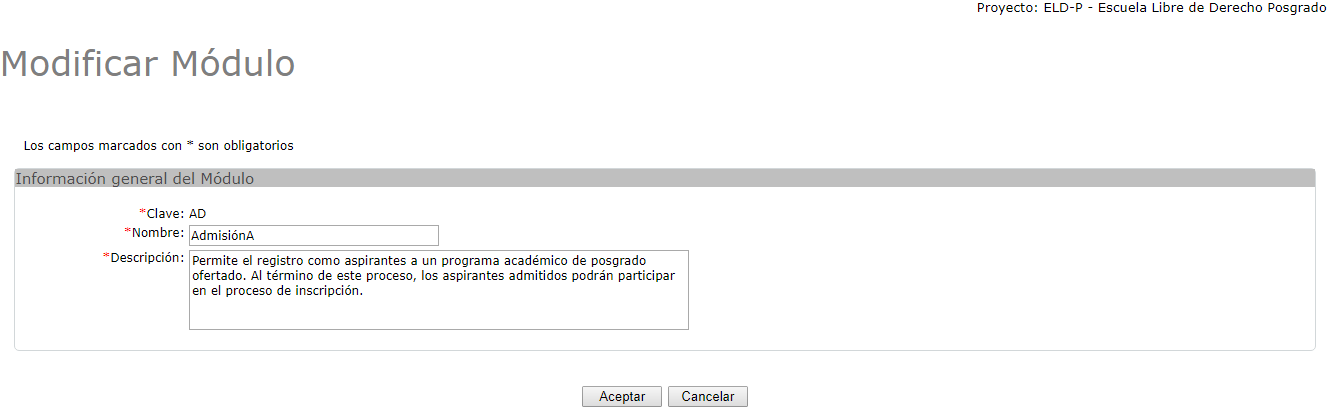
\includegraphics[scale=0.5]{roles/lider/modulos/pantallas/IU5-2modificarModulo}
					\caption{Modificar Módulo}
					\label{fig:modificarModulo}
				\end{center}
			\end{figure}
		
			\item Modifique los datos solicitados por la pantalla.
						
			\item Oprima el botón \IUAceptar.
			
			\item Se mostrará el mensaje \ref{fig:moduloModificado} en la pantalla \ref{fig:GestionarModulos} ''Gestionar Módulos''.
			
			\begin{figure}[htbp!]
				\begin{center}
					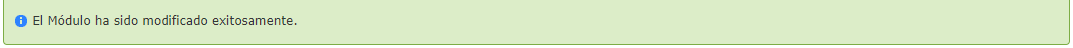
\includegraphics[scale=0.6]{roles/lider/modulos/pantallas/IU5-2MSG1}
					\caption{MSG: Módulo Actualizado}
					\label{fig:moduloModificado}
				\end{center}
			\end{figure}
			\end{enumerate}